\documentclass[11pt,a4paper]{article}
\usepackage[margin=2.2cm]{geometry}
\usepackage{fontspec}
\setmainfont{Palatino}
\setmonofont{Menlo}[Scale=0.82]
\usepackage{graphicx,booktabs,array,xcolor,caption,enumitem,float}
\usepackage[section]{placeins}
\usepackage{tikz}
\usetikzlibrary{positioning,arrows.meta,calc}
\usepackage[hidelinks]{hyperref}
\hypersetup{pdftitle={Multimodal Emotion Recognition on TESS}, pdfauthor={Srivardhan Ginjala}}
\graphicspath{{figures/}}
\captionsetup{font=small,labelfont=bf,labelsep=period,skip=6pt}
\captionsetup[table]{position=top}
\setlist{itemsep=2pt,topsep=4pt}
\renewcommand{\topfraction}{0.85}
\renewcommand{\bottomfraction}{0.6}
\renewcommand{\textfraction}{0.1}
\renewcommand{\floatpagefraction}{0.85}
\newcommand{\code}[1]{\texttt{#1}}
\newcommand{\repo}{gsri-18/MFA-Alignment-and-Multimodal-Emotion-Recognition}
\renewcommand{\arraystretch}{1.2}
\setlength{\emergencystretch}{2em}
\definecolor{blk}{HTML}{E8EEF7}
\definecolor{blkb}{HTML}{4A6FA5}
\definecolor{org}{HTML}{FBEEDD}
\definecolor{orgb}{HTML}{C07A2C}
\tikzset{
  blk/.style={draw=blkb, fill=blk, rounded corners=2pt, align=center, font=\small,
              text width=2.55cm, minimum height=1.45cm, inner sep=3pt},
  fus/.style={draw=orgb, fill=org, rounded corners=2pt, align=center, font=\small,
              text width=2.0cm, minimum height=1.45cm, inner sep=3pt},
  lab/.style={font=\small\bfseries, anchor=east},
  arr/.style={-{Stealth[length=2.2mm]}, thick, draw=black!70},
}

\title{\textbf{Multimodal Emotion Recognition on TESS}\\[2pt]\large Assignment 2b Report}
\author{Srivardhan Ginjala}
\date{November 2026}

\begin{document}
\maketitle

\begin{center}\small
The code, results and report are at \href{https://github.com/\repo}{\texttt{github.com/\repo}}.
\end{center}

\begin{abstract}
\noindent I built speech-only, text-only and multimodal emotion classifiers for the Toronto emotional speech set (TESS)
from frozen WavLM and BERT features with small trained heads. Every TESS clip says ``Say the word \ldots'', so the
transcript is the same for all seven emotions and carries no emotion. On unseen words, speech alone reaches 99.8\%
accuracy, text alone stays at chance (14.3\%) and fusion reaches 99.9\%. On an unseen speaker, speech drops to 65.6\%.
Its learned representation still separates that speaker's emotions, but the decision boundaries learned on the other
speaker do not transfer. Fusion does not help there, and the gated fusion model scores below speech at every seed.
Whisper transcripts carry one clear cue, a question mark on 25\% of the pleasant surprise clips.
\end{abstract}

%=====================================================================
\section{Data and splits}

TESS has 2{,}800 clips from two actresses, OAF (aged 64) and YAF (aged 26). Each speaks the carrier phrase with 200
target words in seven emotions (angry, disgust, fear, happy, neutral, pleasant surprise, sad), giving 400 clips per
emotion. The Kaggle copy contains every file twice, so I deduplicate by file name. One clip is recorded at 96~kHz
instead of 24.4~kHz, so I resample each clip from its own rate.

A random split would place the same word, spoken by the same speaker, in both training and test. I use the two splits
in Table~\ref{tab:splits} instead. All results are the mean and population standard deviation over three seeds.

\begin{table}[htbp]
\centering\small
\caption{The two splits. In the word split, all 14 clips of a word fall in the same part.}
\label{tab:splits}
\begin{tabular}{lcccl}
\toprule
Split & Train & Validation & Test & Evaluates \\
\midrule
\code{word} & 1{,}960 (140 words) & 420 (30 words) & 420 (30 words) & unseen words \\
\code{cross\_speaker} & 1{,}190 (OAF) & 210 (OAF) & 1{,}400 (YAF) & an unseen speaker \\
\bottomrule
\end{tabular}
\end{table}

%=====================================================================
\section{Architecture}

Figure~\ref{fig:arch} shows the blocks of the three pipelines and Table~\ref{tab:blocks} what each contains. The
speech-only and text-only models put the classifier directly after their own branch.

\begin{figure}[htbp]
\centering
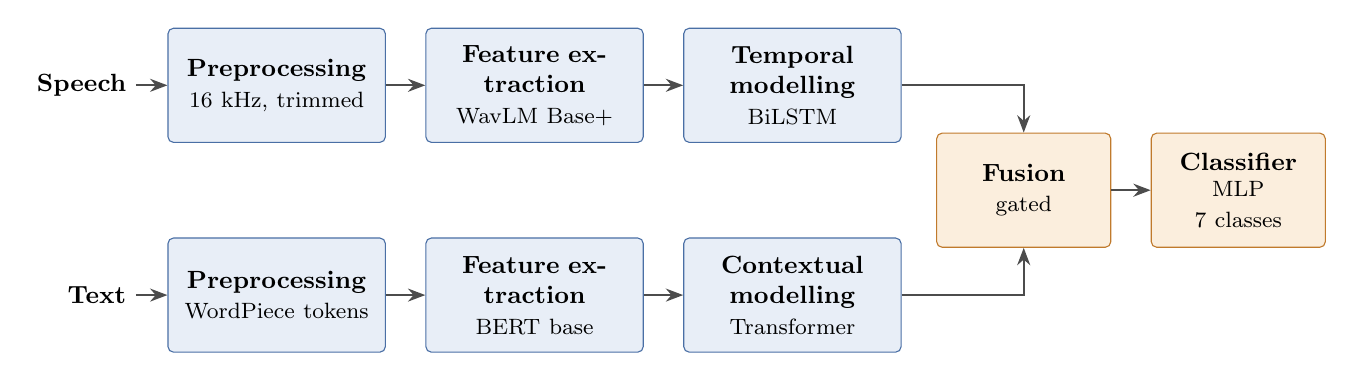
\begin{tikzpicture}[node distance=5mm and 5mm]
  \node[blk] (s1) {\textbf{Preprocessing}\\\footnotesize 16 kHz, trimmed};
  \node[blk, right=of s1] (s2) {\textbf{Feature extraction}\\\footnotesize WavLM Base+};
  \node[blk, right=of s2] (s3) {\textbf{Temporal modelling}\\\footnotesize BiLSTM};
  \node[blk, below=12mm of s1] (t1) {\textbf{Preprocessing}\\\footnotesize WordPiece tokens};
  \node[blk, right=of t1] (t2) {\textbf{Feature extraction}\\\footnotesize BERT base};
  \node[blk, right=of t2] (t3) {\textbf{Contextual modelling}\\\footnotesize Transformer};
  \node[lab, left=4mm of s1] (ls) {Speech};
  \node[lab, left=4mm of t1] (lt) {Text};
  \node[fus] (f) at ($(s3.east)!0.5!(t3.east)+(1.55cm,0)$) {\textbf{Fusion}\\\footnotesize gated};
  \node[fus, right=5mm of f] (c) {\textbf{Classifier}\\\footnotesize MLP\\7 classes};
  \draw[arr] (ls) -- (s1); \draw[arr] (s1) -- (s2); \draw[arr] (s2) -- (s3);
  \draw[arr] (lt) -- (t1); \draw[arr] (t1) -- (t2); \draw[arr] (t2) -- (t3);
  \draw[arr] (s3.east) -| (f.north);
  \draw[arr] (t3.east) -| (f.south);
  \draw[arr] (f) -- (c);
\end{tikzpicture}
\caption{The three pipelines. Each branch produces a 256-dimensional vector. These vectors (temporal, contextual and
fusion) are the representations shown in Figure~\ref{fig:tsne}.}
\label{fig:arch}
\end{figure}

\begin{table}[htbp]
\centering\small
\caption{The blocks of the speech and text branches.}
\label{tab:blocks}
\begin{tabular}{lll}
\toprule
Block & Speech & Text \\
\midrule
Preprocessing & 16 kHz, silence trimmed & Unicode cleanup, WordPiece tokens \\
Features & WavLM Base+, 13 layers, frozen & BERT base, 13 layers, frozen \\
Layer mixing & learned softmax weights & learned softmax weights \\
Modelling & two-layer BiLSTM & two-layer Transformer \\
Pooling & attentive, 256 dimensions & attentive, 256 dimensions \\
\midrule
Fusion & \multicolumn{2}{l}{gated per dimension, with concatenation as a baseline} \\
Classifier & \multicolumn{2}{l}{LayerNorm and a two-layer MLP, the same in all three pipelines} \\
\bottomrule
\end{tabular}
\end{table}

\paragraph{Reasons for each choice.}
\begin{itemize}
\item \textbf{Frozen pretrained encoders.} With 1{,}960 training clips, fine-tuning a 95~M-parameter encoder would
  mostly learn the two voices. Only the heads train (1.1~M parameters for speech, 1.3~M for text, 2.6~M for fusion).
\item \textbf{16~kHz audio with silence trimmed.} WavLM is trained on 16~kHz speech, and trimming keeps the pooling on
  speech. The 4~s cap never cuts a clip, since the longest lasts 2.99~s.
\item \textbf{Per-clip standardisation.} WavLM expects zero mean and unit variance, so the overall level of a clip does
  not reach the model, only the changes of level within it. The log mel baseline keeps the absolute level.
\item \textbf{WavLM Base+.} It is among the strongest base-size models for emotion recognition in the SUPERB benchmark.
  A log mel front end serves as the baseline.
\item \textbf{All 13 layers with learned weights.} Prosody and phonetic content sit in different layers, so the model
  learns which to use.
\item \textbf{A BiLSTM for speech.} It suits clips of 50 to 150 frames and few training examples better than a
  Transformer.
\item \textbf{A light Transformer for text.} BERT's features are already contextual, so two small layers suffice to
  adapt them to the task.
\item \textbf{Attentive pooling.} It weights the frames or tokens that carry emotion, such as a stressed vowel.
\item \textbf{Punctuation kept in the text.} Whisper's question marks turn out to be informative.
\item \textbf{Gated fusion.} The gate weights each modality per clip and per dimension, and its value shows which
  modality the model trusts.
\item \textbf{One classifier for all pipelines.} With the same LayerNorm and MLP everywhere, differences between the
  pipelines come from their representations.
\end{itemize}

\paragraph{Training.} AdamW (learning rate $10^{-3}$, weight decay 0.01), a one-cycle schedule, batch 32 and label
smoothing 0.05, for up to 40 epochs with early stopping on validation macro F1 (patience 10). Each run takes 0.1 to
2.7 minutes on a Colab A100.

%=====================================================================
\section{Results}

Table~\ref{tab:acc} compares all variants over 42 runs (7 variants, 2 splits, 3 seeds).

\begin{table}[htbp]
\centering\small
\caption{Test accuracy and macro F1 (\%), mean $\pm$ population standard deviation over three seeds. Chance is 14.3\%.
The best result of each column is in bold.}
\label{tab:acc}
\begin{tabular}{llcccc}
\toprule
& & \multicolumn{2}{c}{Unseen words} & \multicolumn{2}{c}{Unseen speaker} \\
\cmidrule(lr){3-4}\cmidrule(lr){5-6}
Pipeline & Variant & Accuracy & Macro F1 & Accuracy & Macro F1 \\
\midrule
Speech & WavLM & 99.8 $\pm$ 0.2 & 99.8 $\pm$ 0.2 & \textbf{65.6 $\pm$ 5.8} & \textbf{59.8 $\pm$ 7.1} \\
 & log mel & 99.8 $\pm$ 0.1 & 99.8 $\pm$ 0.1 & 52.2 $\pm$ 2.7 & 48.8 $\pm$ 5.1 \\
\midrule
Text & transcript & 14.3 $\pm$ 0.0 & 4.5 $\pm$ 1.3 & 14.3 $\pm$ 0.0 & 5.9 $\pm$ 1.7 \\
 & Whisper & 19.0 $\pm$ 0.3 & 12.5 $\pm$ 0.5 & 17.0 $\pm$ 0.7 & 13.4 $\pm$ 1.9 \\
\midrule
Fusion & gated & \textbf{99.9 $\pm$ 0.1} & \textbf{99.9 $\pm$ 0.1} & 55.8 $\pm$ 1.6 & 50.4 $\pm$ 1.5 \\
 & concatenated & \textbf{99.9 $\pm$ 0.1} & \textbf{99.9 $\pm$ 0.1} & 55.3 $\pm$ 5.8 & 52.0 $\pm$ 4.4 \\
 & gated, Whisper & \textbf{99.9 $\pm$ 0.1} & \textbf{99.9 $\pm$ 0.1} & 57.5 $\pm$ 11.2 & 55.4 $\pm$ 10.4 \\
\bottomrule
\end{tabular}
\end{table}

\begin{itemize}
\item \textbf{Speech carries the emotion.} Both speech models are almost perfect on unseen words. On the unseen speaker,
  WavLM beats log mel by 13 points.
\item \textbf{Text alone is at chance with the transcript.} With Whisper text it reaches 19\%. Whisper (8.3\% word error
  rate) ends 100 of the 400 pleasant surprise clips with a question mark, and at most 4 clips of any other emotion.
\item \textbf{Fusion does not beat speech.} It matches speech on unseen words. On the unseen speaker the gated model is
  below speech at every seed (its best seed reaches 57.0\%, the worst speech seed 58.7\%). The seed ranges of the other
  two fusion variants overlap with those of speech.
\end{itemize}

%=====================================================================
\section{Analysis}

\subsection{Easiest and hardest emotions}

On unseen words every emotion scores 99.4 to 100\%, so Table~\ref{tab:emo} uses the unseen speaker. Neutral, fear,
sad and disgust transfer well. Angry, happy and pleasant surprise mostly fail.

\begin{table}[htbp]
\centering\small
\caption{Recall per emotion on the unseen speaker (\%), mean over three seeds.}
\label{tab:emo}
\begin{tabular}{lcccc}
\toprule
Emotion & Speech & Text & Fusion & Fusion, Whisper \\
\midrule
neutral & 100.0 & 0.0 & 97.3 & 96.0 \\
fear & 99.3 & 4.7 & 75.5 & 62.5 \\
sad & 96.8 & 0.0 & 75.5 & 93.3 \\
disgust & 92.2 & 38.7 & 83.3 & 66.5 \\
pleasant surprise & 30.5 & 6.2 & 28.8 & 29.2 \\
happy & 21.8 & 17.2 & 21.0 & 45.5 \\
angry & 18.7 & 33.3 & 9.3 & 9.8 \\
\bottomrule
\end{tabular}
\end{table}

Pitch explains part of this (Table~\ref{tab:f0}). The two actresses have almost the same neutral pitch, but YAF's happy
(262~Hz) sits at the level of OAF's angry (267~Hz). The speech model, trained on OAF, labels 309 of YAF's 600 happy
clips as angry over the three seeds (162, 51 and 96), as Figure~\ref{fig:conf} shows for seed 0. The reverse does not
happen. YAF's angry clips go to disgust, fear, neutral and sad and almost never to happy, so pitch level alone does not
explain the errors. Arousal alone does not either, since fear is also high in arousal and transfers at 99.3\%.

\begin{table}[htbp]
\centering\small
\caption{Median F0 (Hz) of 25 clips per speaker and emotion, measured with pYIN.}
\label{tab:f0}
\begin{tabular}{lccc}
\toprule
Speaker & neutral & happy & angry \\
\midrule
OAF (training) & 187 & 236 & 267 \\
YAF (test) & 192 & 262 & 234 \\
\bottomrule
\end{tabular}
\end{table}

\begin{figure}[htbp]
\centering
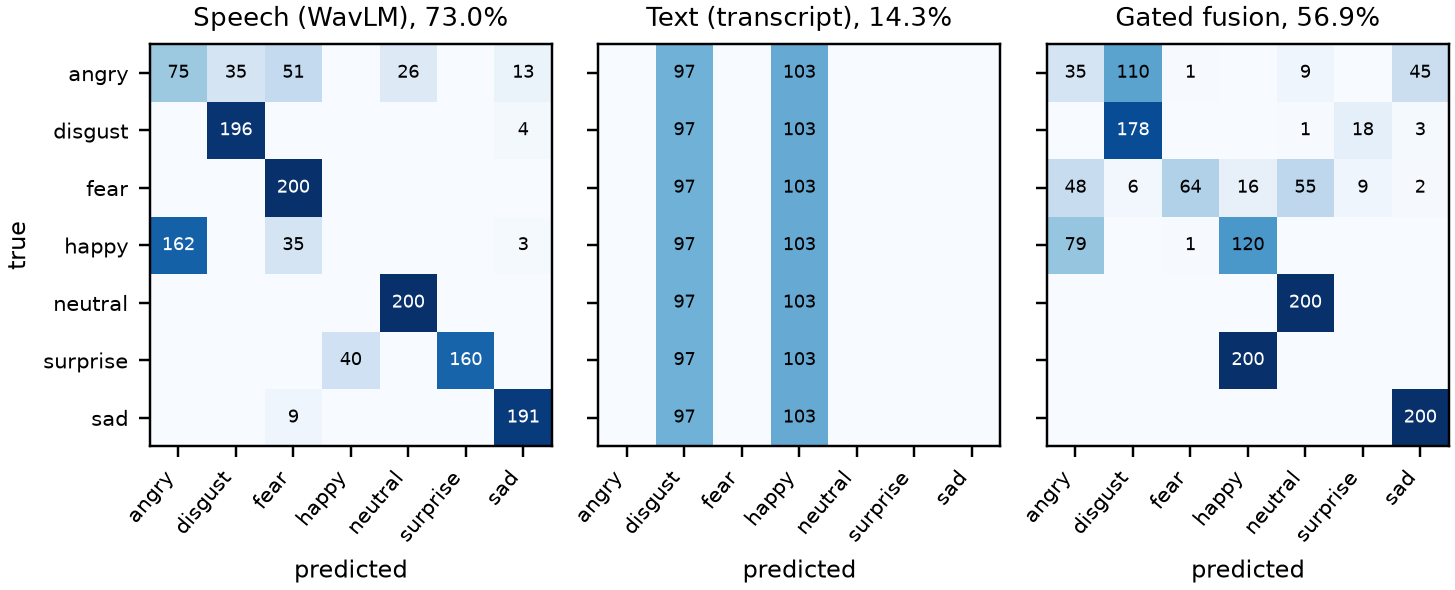
\includegraphics[width=\textwidth]{a2b_confusion.png}
\caption{Confusion matrices on the unseen speaker, seed 0, for speech (WavLM), text (transcript) and gated fusion.
Surprise stands for pleasant surprise. Gated fusion labels all 200 pleasant surprise clips as happy.}
\label{fig:conf}
\end{figure}

\FloatBarrier
\subsection{When does fusion help}

Fusion helps when the second modality adds information, and most when the first is unreliable. The unseen speaker makes
speech unreliable and Whisper adds a little information, yet neither gives a reliable gain (Table~\ref{tab:fusion}).

\begin{table}[htbp]
\centering\small
\caption{Clip-by-clip comparison with speech only at the same seed, summed over three seeds. A gate of 1 keeps only
the speech vector.}
\label{tab:fusion}
\begin{tabular}{llccc}
\toprule
Split & Fusion variant & Errors fixed & Correct answers broken & Mean gate \\
\midrule
Unseen words & gated & 2 & 1 & 0.90 \\
 & gated, Whisper & 2 & 1 & 0.87 \\
 & concatenated & 2 & 1 & n/a \\
\midrule
Unseen speaker & gated & 330 & 741 & 0.87 \\
 & gated, Whisper & 407 & 746 & 0.88 \\
 & concatenated & 344 & 777 & n/a \\
\bottomrule
\end{tabular}
\end{table}

\begin{itemize}
\item \textbf{The transcript gives fusion nothing to use.} Averaged over seeds, the gate gives the speech vector 87 to
  90\% of the weight.
\item \textbf{Validation cannot steer fusion on a new speaker.} The validation clips are OAF, where every speech and
  fusion model reaches a macro F1 of 1.0 (0.995 once), so model selection cannot see how a model will handle YAF. On
  this split the fusion models also stop later (best epoch 5 to 9, against 3 to 4 for the WavLM speech model).
\item \textbf{Whisper text helps two classes.} Compared with fusion on the transcript, it raises happy recall from 21.0
  to 45.5\% and sad from 75.5 to 93.3\% but lowers fear and disgust, and its accuracy ranges from 44 to 72\% across
  seeds.
\item \textbf{Fusion needs words that carry emotion.} It should help on corpora such as IEMOCAP or MELD, where the
  wording itself is emotional. TESS fixes the words by design.
\end{itemize}

\FloatBarrier
\subsection{Error analysis}

The gated fusion model makes no error on unseen words (seed 0), so Table~\ref{tab:fail} lists its five most confident
errors on the unseen speaker, one per confusion pair. All five have a confidence of 0.96 or 0.97, and speech alone was
right in four of them. Figure~\ref{fig:fail} shows each clip next to the same word in the predicted emotion.

\begin{table}[htbp]
\centering\small
\caption{Failure cases of the gated fusion model, seed 0. The true emotion ends the clip name.}
\label{tab:fail}
\begin{tabular}{cllll}
\toprule
\# & Clip & Fusion (confidence) & Speech only & Fusion, Whisper \\
\midrule
1 & \code{YAF\_tire\_angry} & disgust (0.97) & angry & disgust \\
2 & \code{YAF\_yearn\_pleasant\_surprise} & happy (0.96) & pleasant surprise & happy \\
3 & \code{YAF\_bean\_angry} & sad (0.96) & fear & angry \\
4 & \code{YAF\_bath\_fear} & neutral (0.96) & fear & neutral \\
5 & \code{YAF\_jail\_disgust} & pleasant surprise (0.96) & disgust & pleasant surprise \\
\bottomrule
\end{tabular}
\end{table}

\begin{figure}[htbp]
\centering
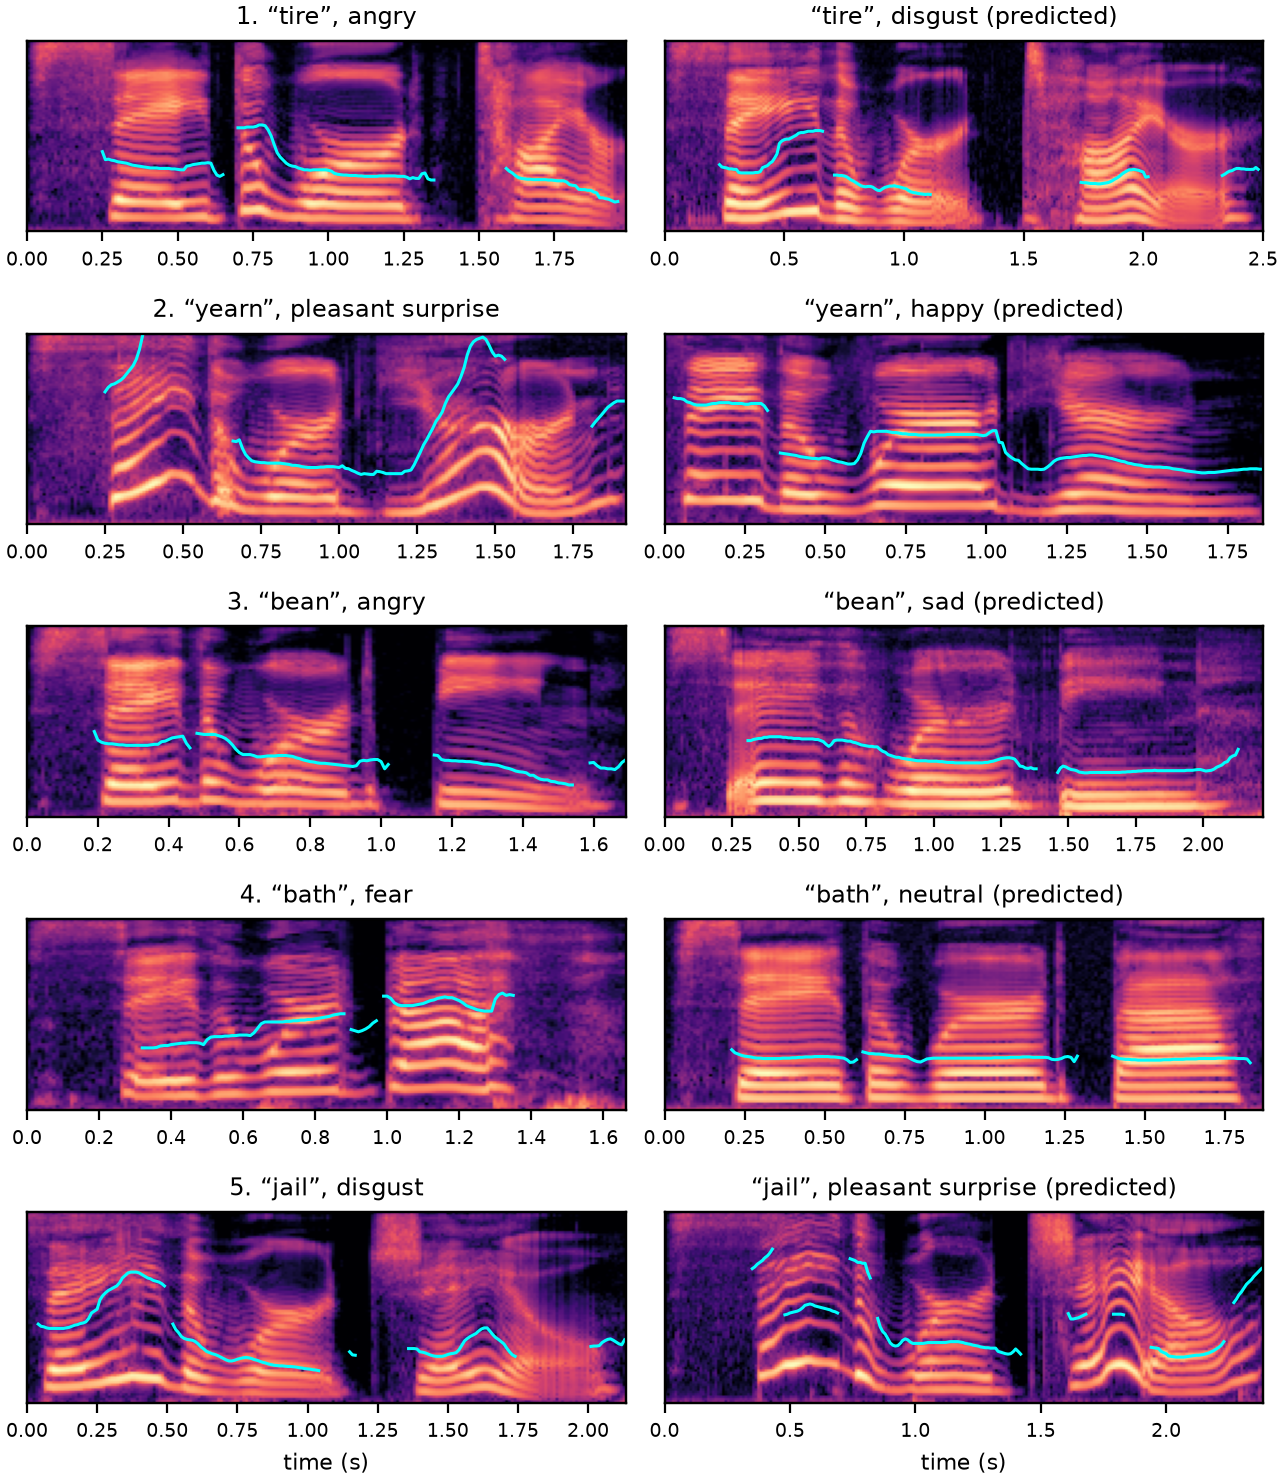
\includegraphics[width=0.74\textwidth]{a2b_failure_cases.png}
\caption{Log mel spectrograms with F0 (cyan, pYIN from 75 to 600~Hz). Left, the misclassified clip. Right, the same word spoken by
YAF in the predicted emotion.}
\label{fig:fail}
\end{figure}

\begin{enumerate}
\item \textbf{Angry as disgust.} Speech alone was right, so the error comes from the layers the fusion model trains and not
  from the frozen WavLM features.
\item \textbf{Pleasant surprise as happy.} F0 peaks at the top of the range on ``say'' and ``yearn'', and YAF's happy is
  also high (262~Hz median).
\item \textbf{Angry as sad.} F0 falls steadily through the phrase with no peak, closer to a sad contour. Speech alone
  also missed this clip.
\item \textbf{Fear as neutral.} Whisper hears ``bath'' as ``Beth'', but fusion with the TESS transcript makes the same
  error, so the transcription is not the cause.
\item \textbf{Disgust as pleasant surprise.} The clip opens with a rise and fall on ``say'' as large as that of the
  surprise clip.
\end{enumerate}

\FloatBarrier
\subsection{Separability of the representations}

Figure~\ref{fig:tsne} shows t-SNE maps of the test vectors from the three blocks, and Table~\ref{tab:sil} their
silhouette scores.

\begin{figure}[htbp]
\centering
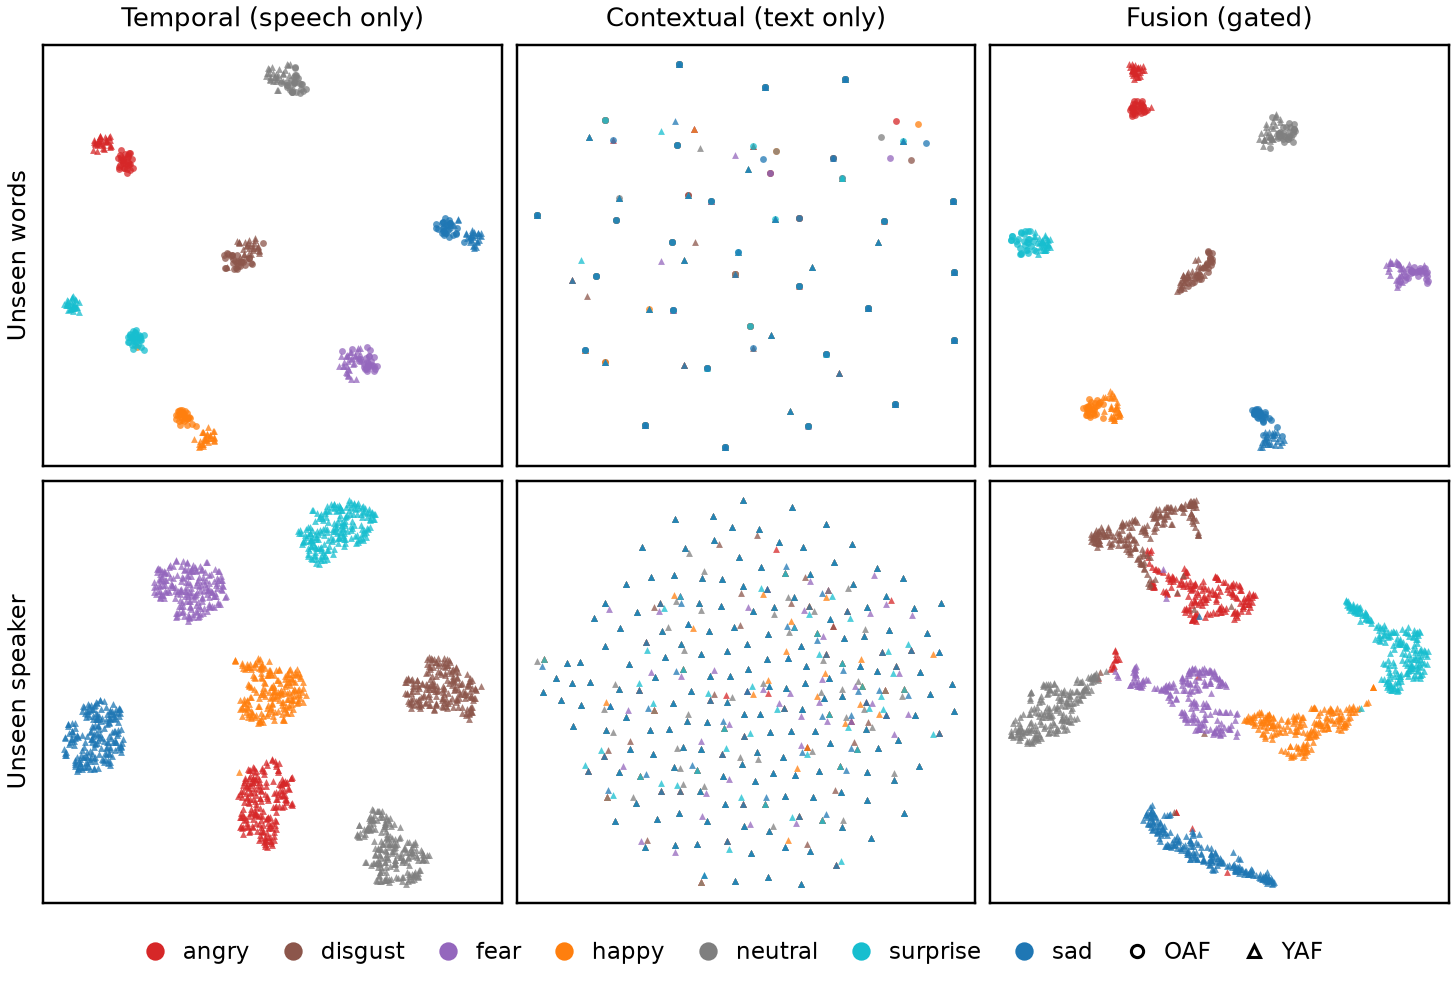
\includegraphics[width=0.9\textwidth]{a2b_tsne.png}
\caption{t-SNE of the test vectors from the temporal block (speech-only model), the contextual block (text-only model,
transcript) and the fusion block (gated fusion model), seed 0. Top, unseen words. Bottom, the unseen speaker, whose
test clips are all YAF. All clips of a word share one transcript and one text vector, so each contextual point hides
several clips.}
\label{fig:tsne}
\end{figure}

\begin{table}[htbp]
\centering\small
\caption{Silhouette scores of the 256-dimensional test vectors, seed 0. A score of 1 means perfectly separated emotions
and 0 means no structure.}
\label{tab:sil}
\begin{tabular}{lccccc}
\toprule
& \multicolumn{3}{c}{Single-modality models} & \multicolumn{2}{c}{Gated fusion model} \\
\cmidrule(lr){2-4}\cmidrule(lr){5-6}
Split & Temporal & Contextual & Contextual, Whisper & Temporal & Fusion \\
\midrule
Unseen words & 0.603 & $-0.017$ & $-0.409$ & 0.824 & 0.893 \\
Unseen speaker & 0.519 & $-0.005$ & $-0.261$ & 0.437 & 0.448 \\
\bottomrule
\end{tabular}
\end{table}

\begin{itemize}
\item \textbf{The temporal block separates the emotions.} It forms one cluster per emotion and speaker on unseen words,
  and one per emotion on the unseen speaker.
\item \textbf{The contextual block shows no emotion structure.} With Whisper text only the clips ending in a question
  mark gather.
\item \textbf{Fusion adds little to its own speech branch.} Inside the fusion model the silhouette rises from 0.824 to
  0.893 on unseen words and from 0.437 to 0.448 on the unseen speaker.
\item \textbf{The unseen speaker clusters cleanly but gets wrong labels.} Its temporal vectors still group by emotion
  (0.519) while the speech model's accuracy is 73\% at seed 0, so the representation transfers and the classifier's
  mapping does not. Per-speaker normalisation or a few labelled clips from the new speaker should close much of the gap.
\end{itemize}

%=====================================================================
\section{Limitations}
\begin{itemize}
\item \textbf{Two speakers.} The unseen-speaker result rests on one direction (OAF to YAF). A corpus with many speakers,
  such as CREMA-D, would allow leave-one-speaker-out evaluation.
\item \textbf{Validation on the training speaker.} It saturates and cannot select models for a new voice. A held-out
  speaker for validation would make model selection meaningful.
\item \textbf{Near-uniform layer weights.} In the best checkpoints of the speech-only models the learned weights stay between
  0.072 and 0.083, around the uniform 0.077, so a higher learning rate for them is worth trying.
\end{itemize}

%=====================================================================
\section{Reproducibility}
\begin{itemize}
\item \textbf{Environment.} Colab A100, Python 3.13, PyTorch 2.14 and transformers 5.22, with the code of commit
  \code{b8e0c73}.
\item \textbf{Data.} The splits (seed 1234) and the Whisper transcripts are in \code{Assignment\_2b/data/}. Both Colab
  sessions produced identical transcripts for all 2{,}800 clips.
\item \textbf{Runs.} A first session finished the 21 runs on unseen words and then ended. A second session restored them
  and ran the other 21 runs and the analysis in 34.7 minutes, and the notebook in \code{colab/} is this second session.
  Every run's log, predictions and metrics are in \code{Assignment\_2b/Results/runs/}.
\item \textbf{Figures.} \code{Report/make\_report\_figures.py} redraws the report figures from these results at print
  size.
\end{itemize}

\end{document}
